The query functions, graph and display functions are integrated into a single graphical front-end relying primarily on the mouse for user input. The graph representation is dynamic and interactive, able to be navigated through by the user in order to obtain detailed information regarding the document database.

\begin{figure}[h]
\centering
\caption{GUI}
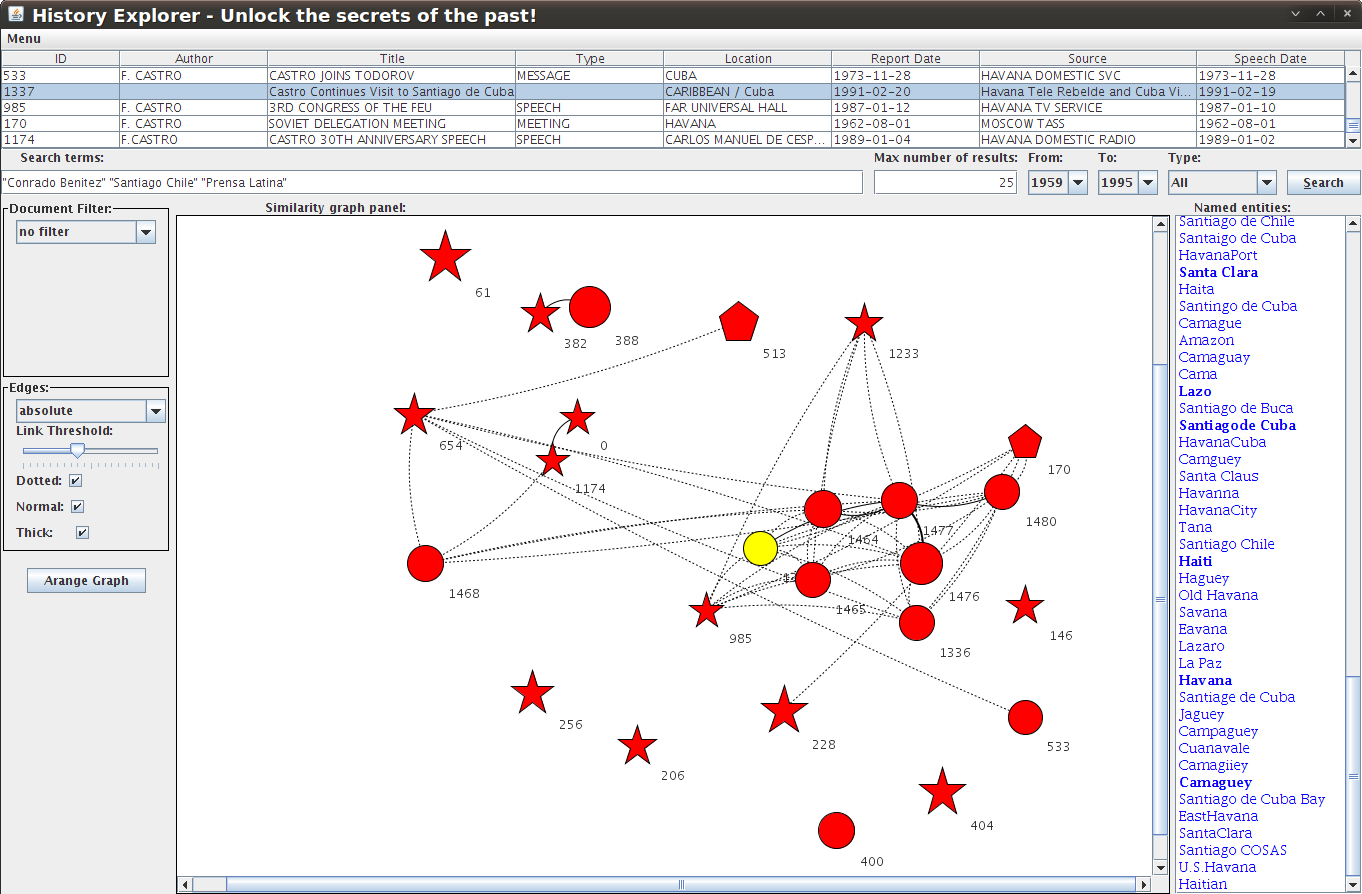
\includegraphics[width=160mm]{gui.png}
\end{figure}

\subsubsection{Search Function}
\begin{figure}[h]
\centering
\caption{Search query}
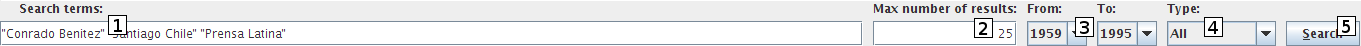
\includegraphics[width=160mm]{search.png}
\end{figure}

Search terms are entered in the query form (item 1 in the figure above)\footnote{Unless otherwise mentioned, the version depicted is \code{2010-04-02}.}: Entering any term will return both NEs and also keywords sharing the exact form (not case-sensitive)--- For instance, entering \lingform{committee} will both return exact instances of \code{committee} in the document itself, and will return NEs similar to \lingform{committee} based on the string kernel similarity measure, e.g.\ \lingform{Central Committee} and \lingform{Central Committee of the Cuban Communist Party}. Multi-word terms are denoted in double quotes, e.g.\ \code{"Central Committee"}. The maximum amount of query results can be adjusted (item 2): For example, entering a value of \code{10} will return ten documents most relevant to the query. The set of years searched between is also modifiable specified by (item 3), as well as the type(s) of documents searched (e.g.\ \code{Speech}, \code{Interview}) (item 5). Once the criteria are entered, the query is run by selecting item 5.

\paragraph{Presentation}
The results of the current query are displayed both in a table of results and in a graph displayed in the main window.

\subsubsection{Results}
\begin{figure}[ht]
\centering
\caption{Query Results Table}
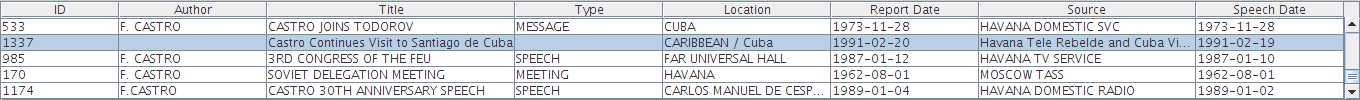
\includegraphics[width=160mm]{table.png}
\end{figure}

In the table, the documents are displayed in rows sorted by their relevance to the query in descending order. The metadata associated with each document is displayed in columns. If there was no metadata retrieved for a document, the entry for the data is empty or \code{NULL}.

\subsubsection{Results}
\begin{figure}[ht]
\centering
\caption{Document Similarity Graph}
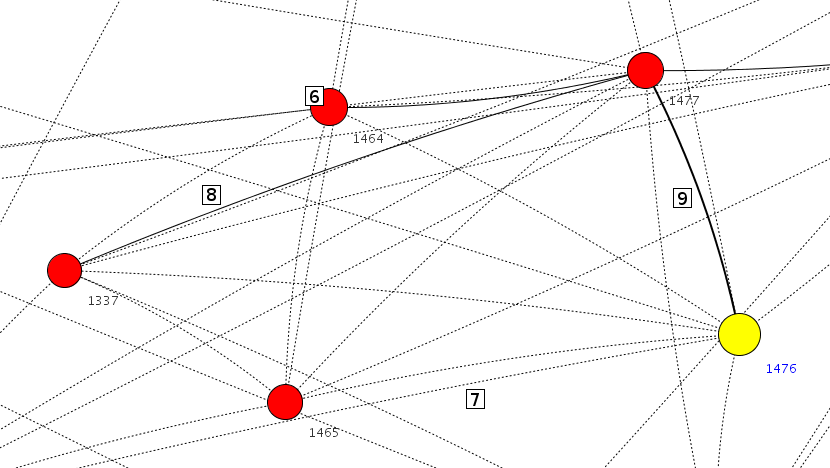
\includegraphics[width=80mm]{nodecloseup.png}
\end{figure}

In the graph, each document is represented by a node (item 6). The relevance of the document to the query is represented by the size of the node: The larger the node, the more relevant the document is to the submitted query. The edges between the nodes represent similarities between the documents based on the similarity of the two documents based on the NEs each contain and their aliases according to the string kernel measure. The stronger the similarity connection, the heavier the line weight of the edge drawn. There are three line weights: ``dotted'' (item 7), ``normal'' (item 8) and ``heavy'' (item 9), in ascending order of the level of similarity they represent. The graph can be scaled in real-time by zooming in and out with the scroll wheel. Furthermore, it is able to re-arrange the position of each node in the graph by clicking and dragging them in order to optimize the view of the graph manually. The graph can also be set to re-arrange the nodes automatically by clicking ``Arrange Graph''. By pressing CTRL and clicking on a node, the view will be centered on the said node automatically.

\paragraph{Navigation}
Selecting a document either through its corresponding entry in the table or node in the graph with the mouse or keyboard highlights it and displays the NEs in the document in a sidebar. The NEs in a particular document and their string kernel-based aliases are displayed in the sidebar: Boldface entries represent NEs in the given document, while the non-boldface entries represent NEs similar to the boldface NEs in the document according to the string kernel similarity measure. For example, the NE \textbf{\lingform{Castro}} may also return the similar NEs \lingform{Fidel}, \lingform{Fidel Castro} and \lingform{Dr.\ Fidel}. The type of the NE (e.g.\ \meta{person} or \meta{organization}) is represented by the color of the text, e.g.\ red for \meta{Persons}, green for \meta{Organizations} and blue for \meta{Locations}. It also is possible to select multiple documents, e.g.\ by holding SHIFT and clicking on multiple nodes/table entries, or by clicking and dragging the mouse to create a selection box encompassing the nodes/table entries to be selected. When multiple documents are selected, the entries displayed in the sidebar are those that are common to all selected documents.

\begin{figure}[ht]
\centering
\caption{Node Context Menu}
\subfloat[][~\hfill{\tiny Version $<$\code{2010-04-02}}]{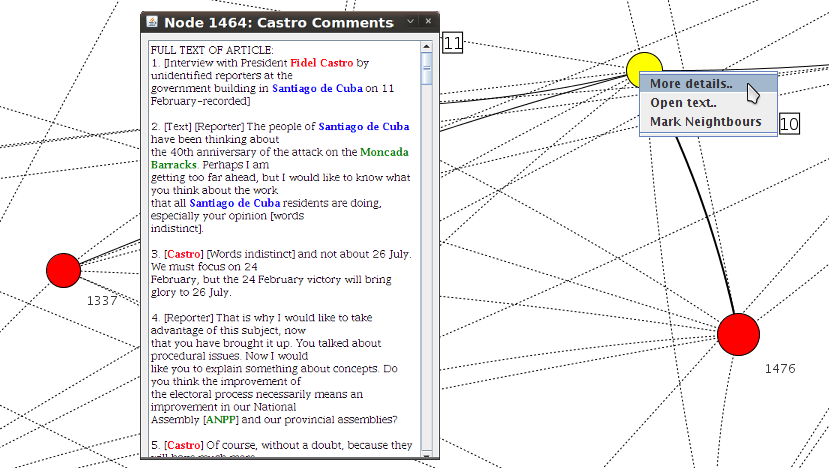
\includegraphics[width=80mm]{nodeclick.png}}
\end{figure}

In addition to viewing document metadata in the query results table, the user may to view the metadata of the document associated with a particular node (e.g.\ document \meta{Type}, \meta{Date} or \meta{Location}) through the node's context menu (item 10) (i.e.\ by right-clicking on the node with the mouse). Also available through the context menu is the text of the document itself, which is displayed in a separate window which can be kept open while still navigating through the graph and viewing other nodes (item 11). The NEs in the text are denoted by being colored according to their type.

\paragraph{\scare{Mark Nearest Neighbors} Function}
Lastly, it is possible through the context menu to automatically select the nearest neighbors of the selected node(s), i.e.\ to select the nodes which share a NE directly with the said node.

\begin{figure}[ht]
\centering
\caption{\scare{Mark Nearest Neighbors} Function}
\subfloat[][Before]{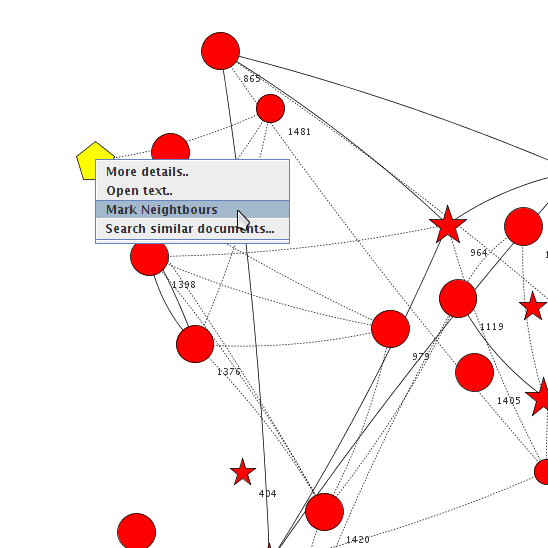
\includegraphics[width=80mm]{markneighbors_before.png}}
\subfloat[][After]{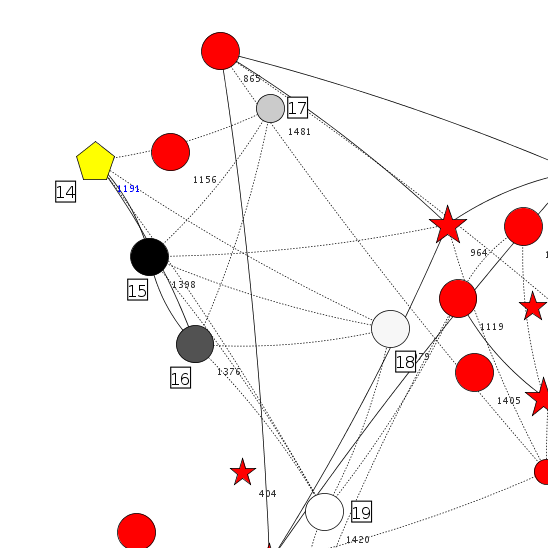
\includegraphics[width=80mm]{markneighbors_after.png}}
\end{figure}

Each nearest neighbor is automatically shaded in a range from black to white to represent the level of similarity between the node and the originally-selected node (item 14): The darker the shade, the more similar the document is to the document of the originally-selected node in relation to the other nearest neighbors; The lighter the shade, the less similar the document is. For example, of the nearest neighbours, item 15 is most similar to the originally-selected node. In descending order of similarity, the next most similar documents are item 16, 17 18 and 19.

\paragraph{Display Options}
\subparagraph{Edge/Node Filtering}

\begin{figure}[ht]
\centering
\caption{Display Options}
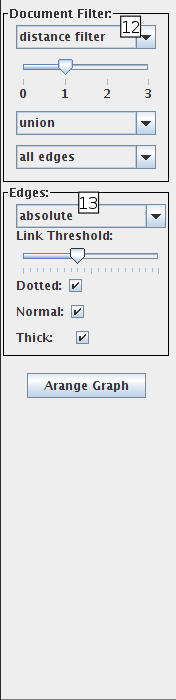
\includegraphics[height=80mm]{displayopts.png}
\end{figure}

The graphical display may be further adjusted by applying a distance filter (item 12) or by adjusting the method by which edges are drawn (item 13).

By default, the edges drawn are determined by the absolute similarity measure: If the similarity measure of two documents is greater than a user-adjustable edge threshold, an edge is drawn between them. The higher the absolute similarity of the two documents, the thicker the edge. However, the user may set the method of edge generation to display edges according to the relative similarity of the documents shown: According to the user-specifiable edge density, the more similar two documents are compared to the similarities of other documents, the thicker the edge.

By adjusting the edge threshold (for absolute similarity) or the edge density (for relative similarity) the user can adjust the level of detail represented by the graph. This allows the user to both discern relationships between documents which are not very similar to each other, and to prune out relatively weaker relationships between documents which are very similar to each other.

Likewise, a vertex filter may be applied, enabling the user to display only nodes of a specified distance $\leq x$ from a selected node or nodes, e.g.\ displaying only the nodes directly connected to the current node(s) (a distance of 1) or displaying nodes which are connected to the selected node through at most one other node (a distance of 2). When selecting multiple nodes, the user can select to display either the union of the neighbors, e.g.\ to display the nodes with a distance of $\leq x$ from \emph{any} selected node, or the intersection of the neighbors, e.g.\ to display only the nodes with a distance of $\leq x$ to \emph{all} selected nodes.

This may be done in real-time, i.e.\ after applying a distance filter, the user may select a node in the graph to view an updated graph of all nodes satisfying the distance criterion for the newly-selected node. This feature allows the user to draw ``sub-graphs'' of the main graph in real time, allowing the user to focus on a particular cluster of documents and thus allowing the user even greater control over the search results.

\subparagraph{Advanced Options}
Finally, for even further control, the user may manually specify all display settings through the \scare{Setup} menu.

\begin{figure}[h]
\centering
\caption{Advanced Settings}
\subfloat[][]{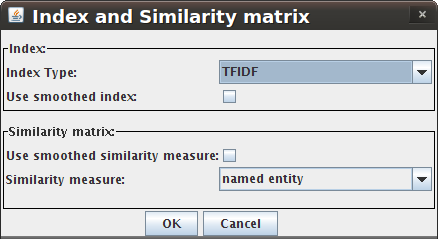
\includegraphics[scale=0.33]{menu_matrices.png}}\quad
\subfloat[][]{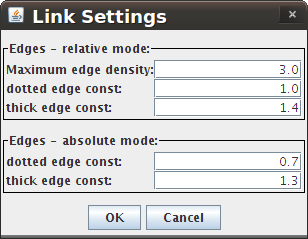
\includegraphics[scale=0.33]{menu_links.png}}\quad
\subfloat[][]{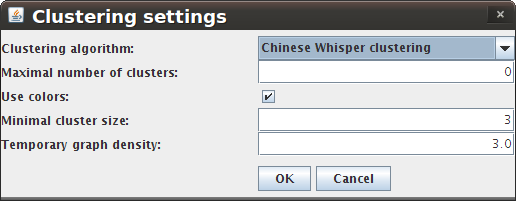
\includegraphics[scale=0.33]{menu_clustering.png}}
\end{figure}

\begin{description}
\item[\scare{Index and Similarity Matrix}] \hfill \\
The user can choose to have document similarities calculated with TF/IDF scores (default) or only TF scores. Additionally, similarities may be calculated with aliasing through the string kernel, or to calculate document similarities with aliasing disabled and associating only exact strings (default). Finally, the similarities can be calculated using only NEs (default), only lexical similarity, or may manually specify the weighting of each measure individually (\scare{custom}), e.g.\ of each type of NE compared to each other and to overall lexical similarity. 
\item[\scare{Link Settings}] \hfill \\
\note{MICHAL}
\item[\scare{Clustering Settings}] \hfill \\
The user can enable CW automatic document clustering (disabled by default), and specify the maximum number of clusters formed, the minimum size of each cluster, as well as the temporary graph density. \note{MICHAL}
\end{description}

All of these features combine to create a powerful interface for searching the corpus and visualizing the results which is both highly automated and highly customizable. In turn, the system is designed to accommodate both basic and advanced users.